\documentclass{article}
\usepackage[margin=2cm]{geometry}
\setlength{\parindent}{0pt}
\usepackage{hyperref}

% Math related
\usepackage{amsmath, bm, amsfonts}
\renewcommand{\vec}[1]{\bm{#1}}
\newcommand{\bhat}[1]{\bm{\hat{#1}}}

% Physics!
% \usepackage{physics}
\newcommand{\iprod}[2]{\langle #1, #2 \rangle}

% Row and Column vectors
\makeatletter
\newcommand\rcvector[2][\\]{\ensuremath{%
  \global\def\rc@delim{#1}%
    \negthinspace\begin{bmatrix}
      \rc@vector #2;\relax\noexpand\@eolst%
    \end{bmatrix}}}
\def\rc@vector #1;#2\@eolst{%
  \ifx\relax#2\relax
    #1
  \else
    #1\rc@delim
    \rc@vector #2\@eolst%
  \fi}
\makeatother

\newcommand{\colvec}{\rcvector}
\newcommand{\rowvec}[1]{\rcvector[,\;]{#1}}

% Graphics related
\usepackage{tikz}

% Other settings
\title{Simple Ball Collision Calculations}
\author{Peleg Bar Sapir}

%% -- BEGIN DOCUMENT -- %%
\begin{document}
\maketitle

%%%%%%%%%%%%%%%%%%%%%%%%%%%
%        BALL-BALL        %
%%%%%%%%%%%%%%%%%%%%%%%%%%%
\section{Ball-Ball Collision}
\subsection{Problem}
Two perfectly spherical $n$-balls ($n\in{2,3}$) with radii $r_{a}, r_{b}$ and masses $m_{a}, m_{b}$ are moving at constant velocities $\vec{u}_{a}, \vec{u}_{b}$. At time $t=0$ their positions are $\vec{x}_{a}, \vec{x}_{b}$. At time $t=\tau$ they collide in an elastic manner.

\vspace{1em}
\underline{2-dimentional illustration of the collision}:
\begin{center}
    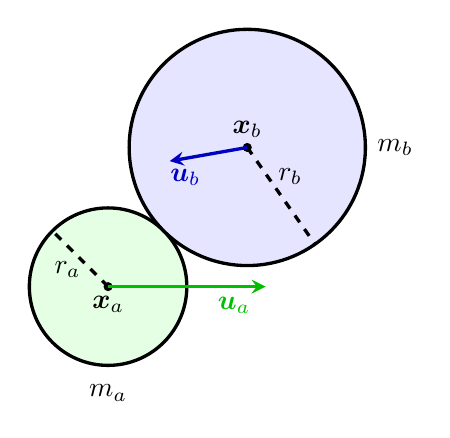
\begin{tikzpicture}
        \tikzset{vector/.style={-stealth, very thick}}
        \pgfmathsetmacro{\angle}{45}
        \pgfmathsetmacro{\ra}{1.0}
        \pgfmathsetmacro{\rb}{1.5}
        \coordinate (xa) at (0,0);
        \coordinate (xb) at ({(\ra+\rb)*cos(\angle)},{(\ra+\rb)*sin(\angle)});
        \draw[very thick, black, fill=green!10] (xa) circle (\ra);
        \draw[very thick, black, fill=blue!10] (xb) circle (\rb);
        \filldraw[black] (xa) circle (0.05) node[below] {$\vec{x}_{a}$};
        \filldraw[black] (xb) circle (0.05) node[above] {$\vec{x}_{b}$};
        \draw[very thick, dashed] (xa) -- (135:\ra) node[pos=0.3, left] {$r_{a}$};
        \draw[very thick, dashed] (xb) -- ++(305:\rb) node[pos=0.3, right] {$r_{b}$};
        \node[below of=xa, yshift=-10pt] {$m_{a}$};
        \node[right of=xb, xshift=25pt] {$m_{b}$};
        \draw[vector, green!75!black] (xa) -- (0:2.0) node[pos=.8, below] {$\vec{u}_{a}$};
        \draw[vector, blue!75!black] (xb) -- ++(190:1.) node[pos=.8, below] {$\vec{u}_{b}$};
    \end{tikzpicture}
\end{center}

\begin{enumerate}
    \item What is the time $t=\tau$ of the collision?
    \item What are the positions $\vec{x}'_{a}, \vec{x}'_{b}$ of the centers of the balls at time $t=\tau$?
    \item What are the velocities $\vec{v}_{a}, \vec{v}_{b}$ immediately following the collision?
\end{enumerate}

\subsection{Solution}

\begin{enumerate}
    \item At the time of collision $t=\tau$ the distance between the balls, $R$ is the sum of their radii:
        \begin{equation}
            R = r_{a} + r_{b}.
            \label{eq:distance_at_collision}
        \end{equation}
        On the other hand, the vector connecting the two balls (i.e. from $\vec{x}_{a}$ to $\vec{x}_{b}$) is
        \begin{equation}
            \Delta \vec{x} = \vec{x}_{a} - \vec{x}_{b} = \colvec{x_{a}^{1}-x_{b}^{1};x_{a}^{2}-x_{b}^{2};\vdots;x_{a}^{n}-x_{b}^{n}},
            \label{eq:pos_diff_vec}
        \end{equation}
        and thus its square length is
        \begin{equation}
            R^{2} = \iprod{\Delta\vec{x}}{\Delta\vec{x}} = \sum\limits_{k=1}^{n}\left(\Delta x^{k}\right)^{2} = \sum\limits_{k=1}^{n}\left(x_{a}^{k}-x_{b}^{k}\right)^{2}.
            \label{eq:dist_sqr}
        \end{equation}
        At each time along their trajectory, the positions of the (center of the) balls are
        \begin{align}
            \vec{x}_{a} &= \tilde{\vec{x}}_{a} + \vec{u}_{a}t,\nonumber\\
            \vec{x}_{b} &= \tilde{\vec{x}}_{b} + \vec{u}_{b}t,
            \label{eq:position_vs_time}
        \end{align}
        where $\tilde{\vec{x}}_{\alpha}$ means the position of the $\alpha$ ball at time $t=0$.
        
        Therefore, at the time of the collision the positions are
        \begin{align}
            \vec{x}_{a} &= \tilde{\vec{x}}_{a} + \vec{u}_{a}\tau,\nonumber\\
            \vec{x}_{b} &= \tilde{\vec{x}}_{b} + \vec{u}_{b}\tau,
            \label{eq:positions_at_collision}
        \end{align}
        which can be written in components form as
        \begin{equation}
            x^{k}_{\alpha} = \tilde{x}^{k}_{\alpha} + u_{\alpha}^{k}\tau. 
            \label{eq:pos_component_form}
        \end{equation}
        
        Subtituting \autoref{eq:pos_component_form} into \autoref{eq:dist_sqr} gives the following expression for $R^2$:
        \begin{equation}
            R^{2} = \sum\limits_{k=1}^{n}\left(\tilde{x}^{k}_{a} + u_{a}^{k}\tau - \tilde{x}^{k}_{b} - u_{b}^{k}\tau\right)^{2} = 
            \label{eq:R_sqr_comp_form}
        \end{equation}

        Combining all similar terms and expanding the parentheses give us an explicit expression for the distance squared in terms of powers of $\tau$:
        \begin{align}
            R^{2} &= \sum\limits_{k=1}^{n}\left(\tilde{x}_{a}^{k}-\tilde{x}_{b}^{k}+\tau\left[u_{a}^{k}-u_{b}^{k}\right]\right)^{2}\nonumber\\
                  &= \sum\limits_{k=1}^{n}\left(\Delta \tilde{x}^{k}+\tau\Delta u^{k}\right)^{2}\nonumber\\
                  &= \sum\limits_{k=1}^{n}\left(\left(\Delta\tilde{x}^{k}\right)^{2}+2\Delta\tilde{x}^{k}\Delta u^{k}\tau + \tau^{2}\left(\Delta u^{k}\right)^{2}\right).
            \label{eq:expanding_R_sqr}
        \end{align}

        Since in \autoref{eq:expanding_R_sqr} we have a sum of three expressions in each term, we can rewrite it as
        \begin{equation}
            R^{2} = \sum\limits_{k=1}^{n}\left(\Delta\tilde{x}^{k}\right)^{2} + 2\tau\sum\limits_{k=1}^{n}\Delta\tilde{x}^{k}\Delta u^{k} + \tau^{2}\sum\limits_{k=1}^{n}\left(\Delta u^{k}\right)^{2}.
            \label{eq:many_sums}
        \end{equation}

        Now each of these sums can be viewed in terms of an inner product:
        \begin{equation}
            R^{2} = \iprod{\Delta\tilde{\vec{x}}}{\Delta\tilde{\vec{x}}} + 2\tau\iprod{\Delta\tilde{\vec{x}}}{\Delta\vec{u}} + \tau^{2}\iprod{\Delta\vec{u}}{\Delta\vec{u}}.
            \label{eq:sums_to_inner_prods}
        \end{equation}

        This is a simple quadratic equation in $\tau$, with 
        \begin{align}
            a &= \iprod{\Delta{\vec{u}}}{\Delta{\vec{u}}},\nonumber\\
            b &= 2\iprod{\Delta\tilde{\vec{x}}}{\Delta{\vec{u}}},\nonumber\\
            c &= \iprod{\Delta\tilde{\vec{x}}}{\Delta\tilde{\vec{x}}} - R^{2}.
            \label{eq:quadratic}
        \end{align}

        For \autoref{eq:sums_to_inner_prods} to have a real solution, the first condition is that $b^{2}-4ac\geq0$, or
        \begin{equation}
            \iprod{\Delta\tilde{\vec{x}}}{\Delta{\vec{u}}}^{2} \geq \iprod{\Delta{\vec{u}}}{\Delta{\vec{u}}}\iprod{\Delta\tilde{\vec{x}}}{\Delta\tilde{\vec{x}}} - R^{2}.
            \label{eq:test}
        \end{equation}

    \item The positions of the balls at the time of impact can be found by subtituting $t=\tau$ into \autoref{eq:positions_at_collision}:
        \begin{align}
            \vec{x}_{a} &= \tilde{\vec{x}}_{a} + \vec{u}_{a}\tau,\nonumber\\
            \vec{x}_{b} &= \tilde{\vec{x}}_{b} + \vec{u}_{b}\tau,
            \label{eq:positions_at_collision_2}
        \end{align}

    \item \underline{Note}: the solution given here is based on the text in \href{https://www.sjsu.edu/faculty/watkins/collision.htm}{this webpage}.

        \vspace{1em}
        Conservation of momentum gives
        \begin{equation}
            m_{a}\vec{u}_{a} + m_{b}\vec{u}_{b} = m_{a}\vec{v}_{a} + m_{b}\vec{v}_{b},
            \label{eq:conservation_of_momentum_1}
        \end{equation}
        i.e.
        \begin{equation}
            m_{a}\left(\vec{u}_{a}-\vec{v}_{a}\right) = -m_{b}\left(\vec{u}_{b}-\vec{v}_{b}\right).
                            \label{eq:conservation_of_momentum_2}
        \end{equation}

        Conservation of (kinetic) energy gives
        \begin{equation}
            \frac{1}{2}m_{a}u_{a}^{2} + \frac{1}{2}m_{b}u_{b}^{2} = \frac{1}{2}m_{a}v_{a}^{2} + \frac{1}{2}m_{b}v_{b}^{2},
            \label{eq:conservation_of_energy_1}
        \end{equation}
        which can be further simplified using the dot product (since for any vector $\vec{w}$, $w^{2}=\vec{w}\cdot\vec{w}$) and eliminating the $\frac{1}{2}$ coefficient, leaving us with
        \begin{equation}
            m_{a}\left( \vec{u}_{a}\cdot\vec{u}_{a} - \vec{v}_{a}\cdot\vec{v}_{a} \right) = -m_{b}\left( \vec{u}_{b}\cdot\vec{u}_{b} - \vec{v}_{b}\cdot\vec{v}_{b} \right),
            \label{eq:conservation_of_energy_2}
        \end{equation}
        i.e. (utilizing $a^{2}-b^{2}=(a-b)(a+b)$)
        \begin{equation}
            m_{a}\left( \vec{u}_{a}-\vec{v}_{a} \right)\cdot\left( \vec{u}_{a}+\vec{v}_{a} \right) = m_{b}\left( \vec{u}_{b}-\vec{v}_{b} \right)\cdot\left( \vec{u}_{b}+\vec{v}_{b} \right).
            \label{eq:conservation_of_energy_3}
        \end{equation}

        The change in momentum must happen along the line connecting the centers of the balls. We can easily derive the vector connecting $\vec{x}_{b}$ to $\vec{x}_{a}$:
        \begin{equation}
            \vec{x} = \vec{x}_{a}-\vec{x}_{b},
            \label{eq:connect_x1_x2}
        \end{equation}
        and normalize it to
        \begin{equation}
            \bhat{X} = \frac{\vec{x}_{a}-\vec{x}_{b}}{\left\|\vec{x}_{a}-\vec{x}_{b} \right\|} = \frac{\vec{x}}{r_{a}+r_{b}}.
            \label{eq:unit_connect_x1_x2}
        \end{equation}

        The change in momentum is this given by
        \begin{equation}
            m_{a}\left( \vec{u}_{a}-\vec{v}_{a} \right) = -m_{b}\left( \vec{u}_{b}-\vec{v}_{b} \right) = \alpha\bhat{X},
            \label{eq:change_in_momentum}
        \end{equation}
        where $\alpha\in\left(0, \infty\right)$.

        We can use \autoref{eq:change_in_momentum} to express \autoref{eq:conservation_of_energy_3} as
        \begin{equation}
            \bhat{X}\cdot\left(\vec{u}_{a}+\vec{v}_{a}\right) = \bhat{X}\cdot\left(\vec{u}_{b}+\vec{v}_{b}\right),
            \label{eq:label}
        \end{equation}
        and using \autoref{eq:change_in_momentum} we get the following expressions for the velocities $\vec{v}_{i}$:
        \begin{align}
            \vec{v}_{a} &= \vec{u}_{a} - \frac{\alpha}{m_{a}}\bhat{X},\nonumber\\
            \vec{v}_{b} &= \vec{u}_{b} + \frac{\alpha}{m_{b}}\bhat{X}.
            \label{eq:v_from_u}
        \end{align}

        The only thing left to do is to find $\alpha$. Applying \autoref{eq:v_from_u} to \autoref{eq:conservation_of_energy_3} we find that
        \begin{equation}
            \bhat{X}\cdot\left(2\vec{u}_{a}-\frac{\alpha}{m_{a}}\bhat{X}\right) = \bhat{X}\left(2\vec{u}_{b}+\frac{\alpha}{m_{b}}\bhat{X}\right).
            \label{eq:find_alpha}
        \end{equation}
        and since $\bhat{X}$ is a unit vector, i.e. $\bhat{X}\cdot\bhat{X}=1$, the above reduces to
        \begin{equation}
        2\bhat{X}\cdot\left(\vec{u}_{a}-\vec{u}_{b}\right) = \alpha\left(\frac{1}{m_{a}}+\frac{1}{m_{b}}\right),
            \label{eq:reduction_1}
        \end{equation}
        and thus
        \begin{equation}
        \alpha = \frac{2\bhat{X}\left(\vec{u}_{a}-\vec{u}_{b}\right)}{\frac{1}{m_{a}}+\frac{1}{m_{b}}}.
            \label{eq:reduction_2}
        \end{equation}

        To simplify things further, we can define two more quantities:
        \begin{align}
            \Delta \vec{u} &= \vec{u}_{a}-\vec{u}_{b},\\
            \mu &= \frac{1}{\frac{1}{m_{a}}+\frac{1}{m_{b}}},
            \label{eq:simplifications_1}
        \end{align}
        and then \autoref{eq:reduction_2} simplifies to
        \begin{equation}
            \alpha = 2\mu\bhat{X}\Delta\vec{u}.
            \label{eq:simplifications_2}
        \end{equation}
\end{enumerate}

%%%%%%%%%%%%%%%%%%%%%%%%%%%
%        Ball-Wall        %
%%%%%%%%%%%%%%%%%%%%%%%%%%%
\section{Ball-Wall Collision}
\subsection{Problem}
Given a single ball moving with a constant velocity $\vec{u}$ and a wall defined as a rectangular cut of a plane with normal $\bhat{n}$ and containing the point $\vec{p}$ -

\begin{enumerate}
    \item will the ball collide with the wall at any time $t\geq0$?
    \item If there is a collision - at what point in space and at what time does it occur, and
    \item what is the velocity $\vec{v}$ of the ball immediately following the collision?
\end{enumerate}

\subsection{Solution}
\begin{enumerate}
    \item We will use the following steps to check for collision between a ball and a wall: first we check if there is an intersection between the wall's (infinite) plane and the line defined by the ball's position and velocity. If the intersection doesn't happens in the past, we will check if the intersection point is within the rectangular section of the plane. (figure?)

        The position of the ball as a function of time is given by \autoref{eq:position_vs_time}. Adjusting to this section it is
        \begin{equation}
            \vec{x}(t) = \vec{x} + \vec{u}t,
            \label{eq:position_vs_time_ball_wall}
        \end{equation}
        where $\vec{x}$ is the initial position of the ball and $t\in\mathbb{R}$. On the other hand, the equation defining the entire (infinite) plane of the wall is given by the set of all points $\vec{p}$ for which
        \begin{equation}
            \left(\vec{p}-\vec{p}_{0}\right)\cdot \bhat{n} = 0,
            \label{eq:wall_plane}
        \end{equation}
        where $\vec{p}_{0}$ is any \textit{known} point on the plane and $\bhat{n}$ is the normal to the plane. Subtituting \autoref{eq:position_vs_time_ball_wall} into \autoref{eq:wall_plane} we get
        \begin{equation}
            \left(\left(\vec{x}+\vec{u}t\right)-\vec{p}_{0}\right)\cdot\bhat{n} = 0.
            \label{eq:line_plane_1}
        \end{equation}
        
        Expanding and solving for $t$ we get
        \begin{equation}
            t = \frac{\left(\vec{p}_{0}-\vec{x}\right)\cdot\bhat{n}}{\vec{u}\cdot\bhat{n}}.
            \label{eq:line_plane_2}
        \end{equation}

        If $\vec{u}\cdot\bhat{n}=0$ then the ball is moving at a trajectory parallel to the wall. If $\vec{u}\cdot\bhat{n}\neq0$ then $t$ is a real number, and we need to check whether it is larger than or equal to $0$ (i.e. validating that the collision didn't happen in the past) and whether the.
\end{enumerate}

\end{document}
